\section{Описание}

В качестве датасета я выбрал \enquote{Heart Attack Analysis \& Prediction Dataset} с сайта kaggle.\\
Он находится по ссылке https://www.kaggle.com/datasets/rashikrahmanpritom/heart-attack-analysis-prediction-dataset?select=heart.csv. \\В данном датасете собраны некоторые признаки, влияющие на возникновение сердечного приступ.\\

В этом наборе данных приведены признаки:\\

\begin{enumerate}
 \item Age : Возраст пациента
 \item Sex: Пол пациента
 \item exang: стенокардия, вызванная физической нагрузкой (1 = да; 0 = нет)
 \item cp: тип боли в груди
	\begin{enumerate}
	 \item Value 1: типичная стенокардия
	 \item Value 2: атипичная стенокардия
	 \item Value 3: неангинальная боль
	 \item Value 4: бессимптомное течение
	\end{enumerate}
 \item trtbps: артериальное давление в состоянии покоя (в мм рт. ст.)
 \item chol: холесторал в мг / дл, определяемый с помощью датчика ИМТ
 \item fbs: (уровень сахара в крови натощак> 120 мг / дл) (1 = истина; 0 = ложь)
 \item rest\_ecg : результаты электрокардиографии в состоянии покоя
	\begin{enumerate}
	 \item Value 0: нормальное
	 \item Value 1: аномалия зубца ST-T (инверсия зубца T и / или повышение или понижение ST> 0,05 мВ)
  	 \item Value 2: отображение вероятной или определенной гипертрофии левого желудочка по критериям Эстеса
	\end{enumerate}
 \item thalach: достигнутая максимальная частота сердечных сокращений
 \item target : 0 = меньше шансов сердечного приступа 1 = больше шансов сердечного приступа
\end{enumerate}

В данной лабораторной работе реализованы следующие алгоритмы обучения:

1) k-Nearest Neighbors (KNN)
Идея заключается в определении класса объекта по классам k ближайших(каких
больше - такой и класс).

2) Naive Bayes
Построен на формуле Байеса  $ P(A|B)=  \frac{P(B|A)∗P(A) } {P(B)} $

3)Linear / Logistic Regression
Попытка провести разделяющую гиперплоскость между классами

4)SVM
Линейная с дополнительным условием: максимизируется расстояние от объектов до
гиперплоскости




\pagebreak

\section{Ход работы}

\CWHeader{KNN}

Проведем те же манипуляции с датасетом что и в лабораторной работе № 0.\\
Далее начнем обучать модели.

Сначала обучим модель KNN. Её код приведен ниже.

\begin{lstlisting}[language=C]
class KNN(BaseEstimator, ClassifierMixin):
    def __init__(self, k):
        self.k = k
        
    def fit(self, data, labels):
        self.data = data
        self.labels = labels
        
    def euclidean_distance(self, data, row):
        distance = 0
        for i in range(len(data)): 
            distance += (data[i] - row[i]) ** 2
        return math.sqrt(distance)
        
    def predict(self, dataX):
        res = np.ndarray((dataX.shape[0],))
        for j, data in enumerate(dataX):
            distances = []
            for i, row in enumerate(self.data):
                distances.append((self.euclidean_distance(data, row), self.labels[i]))
            distances.sort(key = lambda tup: tup[0])
            dictionary = collections.defaultdict(int)
            for i in range(self.k):
                dictionary[distances[i][1]] += 1
            res[j] = max(dictionary.items(), key = lambda tup: tup[1])[0]
        return res
\end{lstlisting}

\begin{alltt}
\{'knn\_\_k': 3\}
Accuracy train: 0.6697278911564626
Accuracy: 0.5737704918032787
Recall: 0.7307692307692307
Precision: 0.5
\end{alltt}

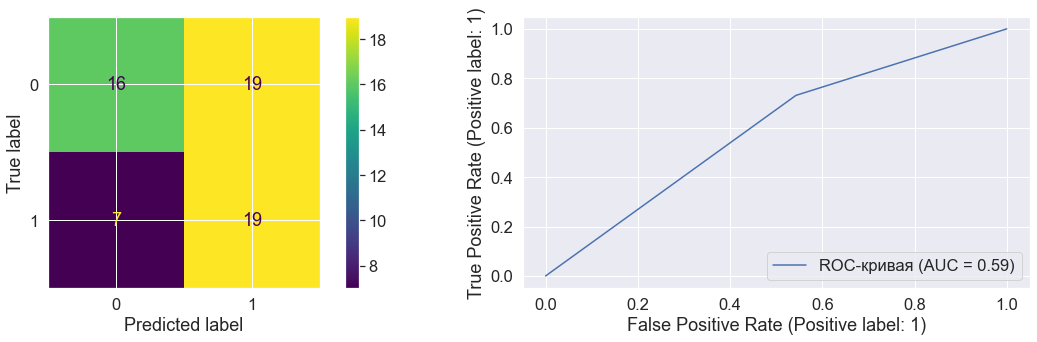
\includegraphics[width=\textwidth]{myknn} 

Все классы наследуем от BaseEstimator и ClassifierMixin. Соответвенно реализовано две основные функции: fit, обучающая модель на
тренировочных данных, в этом алгоритме данная функция только сохроняет данные, и predict, которая уже непосредственно выдает результат для
тестовых данных. В качестве меры используем классическое расстояние Евклида.
Из результатов видно, что точность крайне низкая, вероятно, потому что точки на графике находятся одним облаком и их сложно отличить друг от друга данным алгоритмом.

\begin{alltt}
\{'knn\_\_n\_neighbors': 3\}
Accuracy train: 0.6697278911564626
Accuracy: 0.5737704918032787
Recall: 0.7307692307692307
Precision: 0.5
\end{alltt}
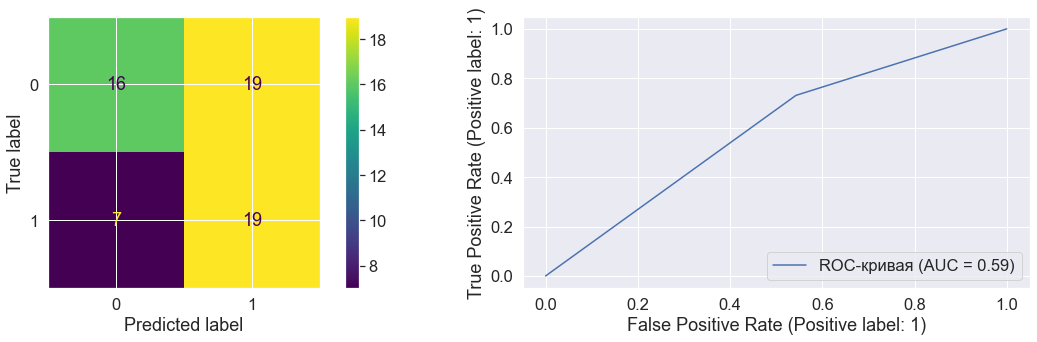
\includegraphics[width=\textwidth]{sklknn}

Точность, полученная с помощью коробочного решения, равна точности, полученной с помощью моего решения. Значит проблема действительно а датасете.


\CWHeader{NaiveBayes}

\begin{lstlisting}[language=C]
class NaiveBayes(BaseEstimator, ClassifierMixin):
    def __init__(self, bins):
        self.bins = bins
        pass
    
    def fit(self, data, labels):
        self.data = data
        self.labels = labels
        self.classes = []
        for j in np.unique(labels):
            
            self.classes.append([])
            for i in range (data.shape[1]):
                self.classes[j].append([*np.histogram(data[labels == j, i], bins = self.bins)])
                self.classes[j][-1][0] = self.classes[j][-1][0].astype('float64') / len(data[labels == j, i])
        
        self.prclasses = np.unique(labels, return_counts = True)[1] / len(labels)
        
    def predict(self, maindata):
        res = np.ndarray((maindata.shape[0],))
        for j, data in enumerate(maindata):
            maximum = 0
            ans = 0
            for i in range(len(self.classes)):
                p = self.prclasses[i]
                for k in range(len(self.classes[i])):
                    ind = np.digitize(data[k], self.classes[i][k][1])
                    
                    if ind >= len(self.classes[i][k][1]) or ind <= 0:
                        p = 0
                    else:
                        p *= self.classes[i][k][0][ind - 1]
                    
                if p > maximum:
                    maximum = p
                    ans = i
            res[j] = ans
        return res 
\end{lstlisting}

\begin{alltt}
\{'bn\_\_bins': 8\}
Accuracy train: 0.7812925170068027
Accuracy: 0.7868852459016393
Recall: 0.8461538461538461
Precision: 0.7096774193548387
\end{alltt}

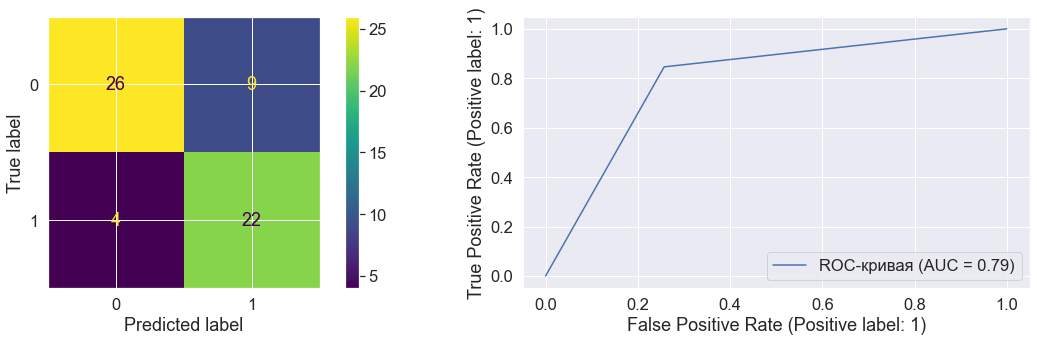
\includegraphics[width=\textwidth]{mynb} 

Приемлимую точность удалось получить при помощи алгоритма Байесовского классификатора. Из тепловой карты видно, что многие велечины почти не коррелируют друг с другом, поэтому наивное предположение об условной независимости между каждой парой характеристик при заданном значении переменной класса вместе с методом Байеса дает высокую точность. Также распределение признаков похоже на нормальное, это тоже дает плюс Байесовскому классификатору.

\begin{alltt}
Accuracy: 0.7868852459016393
Recall: 0.7692307692307693
Precision: 0.7407407407407407
\end{alltt}
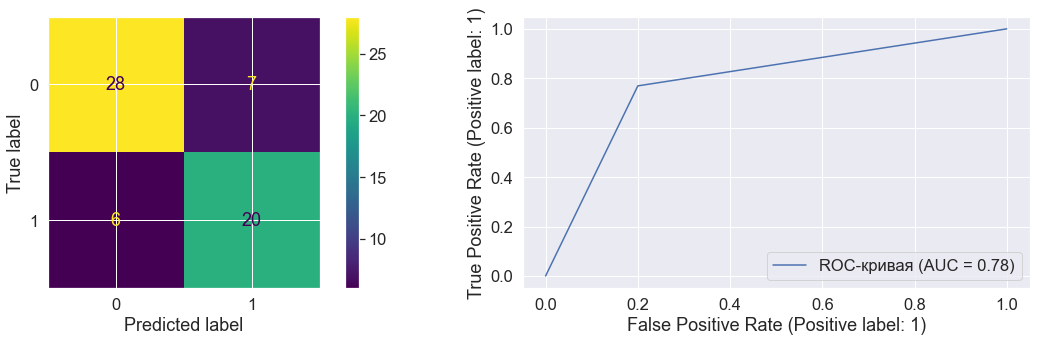
\includegraphics[width=\textwidth]{sklnb}

Примерно такой же точности достигает коробочное решение.


\CWHeader{Logistic Regression }

\begin{lstlisting}[language=C]
class Logistic(BaseEstimator, ClassifierMixin):
    def __init__(self, lr, nepoch, batch_size):
        self.lr = lr
        self.nepoch = nepoch
        self.batch_size = batch_size
        pass
    
    def sigmoid(self, x):
        self.l = 1 / (1 + np.exp(-x))
        return self.l
        
    def fit(self, data, labels):
        data = np.concatenate((data, np.ones((data.shape[0],1))), axis = 1)
        self.W = np.random.normal(0, 1, (len(data[0]),))
        
        for i in range(self.nepoch):
            for i in range(0, len(data), self.batch_size):
                xb = data[i:i + self.batch_size]
                yb = labels[i:i + self.batch_size]
                p = np.dot(self.W, xb.T)
                s = self.sigmoid(p)
                dp = np.dot(xb.T, (s - yb).T)
                self.W -= self.lr * dp
        
    def predict(self, maindata):
        maindata = np.concatenate((maindata, np.ones((maindata.shape[0],1))), axis = 1)
        p = np.dot(self.W, maindata.T)
        s = self.sigmoid(p)
        return (s > 0.5).astype('int64')
\end{lstlisting}

В данном методе на вход подается 3 параметра: размер батча(batch_size) - размер «пачки», которую будет обрабатывать модель, коэффициент обучения(lr) - скорость градиентного
спуска и количество эпох(nepoch) - сколько раз мы будет прогонять модель по одним
и тем же данным. Параметры модели - матрица W, на которую мы будем умножать.
Так как функция должна выглядеть, как Wx + b, увеличим размерность W и x на 1,
добавив туда тем самым b. В качестве функции ошибки используется log loss. Также
используется функция sigmoid для интепретации вывода результатов модели.

\begin{alltt}
\{'log\_\_batch\_size': 1, 'log\_\_lr': 0.1, 'log\_\_nepoch': 20\}
Accuracy train: 0.6282312925170068
Accuracy: 0.5573770491803278
Recall: 0.9615384615384616
Precision: 0.49019607843137253
\end{alltt}


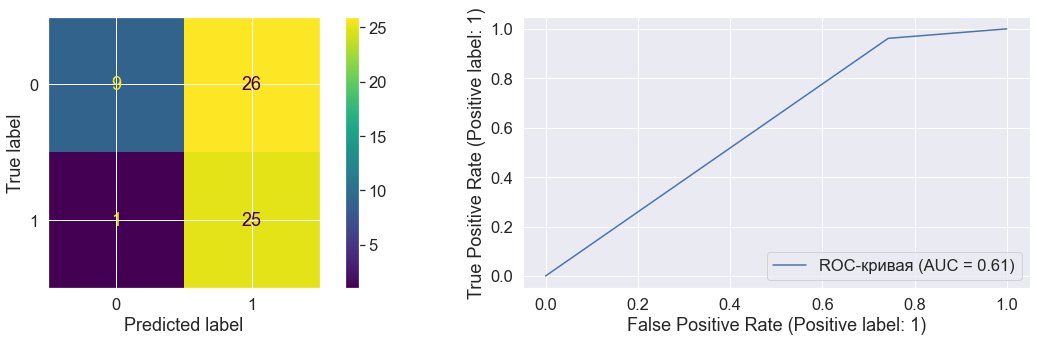
\includegraphics[width=\textwidth]{mylog} 

\begin{alltt}
\{'log\_\_alpha': 0.001, 'log\_\_max_iter': 100\}
Accuracy train: 0.6656462585034014
Accuracy: 0.6557377049180327
Recall: 0.7307692307692307
Precision: 0.5757575757575758
\end{alltt}
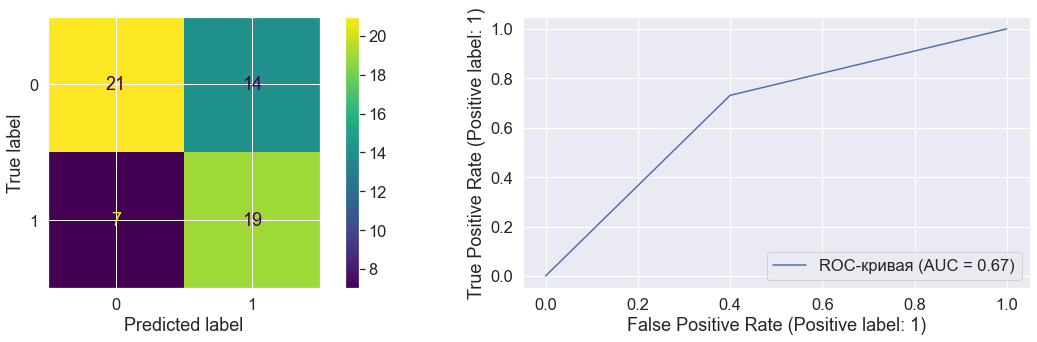
\includegraphics[width=\textwidth]{skllog}

Точность снова низкая у обоих вариантов реализации. Это происходит из-за того что данные плохо разделяются линией.


\CWHeader{SVM}

\begin{lstlisting}[language=C]
class SVM(BaseEstimator, ClassifierMixin):
    def __init__(self, lr, lambd,  batch_size, nepoch):
        self.nepoch = nepoch
        self.lr = lr
        self.lambd = lambd
        self.batch_size = batch_size
        
    def fit(self, data, labels):
        data = np.concatenate((data, np.ones((data.shape[0],1))), axis=1)
        self.W = np.random.normal(0, 1, (len(data[0]),))
        
        for i in range(self.nepoch):
            for i in range(0, len(data), self.batch_size):
                xb = data[i:i + self.batch_size]
                yb = labels[i:i + self.batch_size]
                
                p = np.dot(self.W, xb.T)

                sums = np.zeros_like(self.W)
                for i in range(len(p)):
                    if 1 - p[i] * yb[i] > 0:
                        sums -= xb[i] * yb[i]

                dp = 2 * self.lambd * self.W + sums
                self.W -= self.lr * dp
                
                
    def predict(self, maindata):
        maindata = np.concatenate((maindata, np.ones((maindata.shape[0],1))), axis=1)
        p = np.dot(self.W, maindata.T)
        return np.sign(p)
\end{lstlisting}


\begin{alltt}
\{'lin\_\_batch\_size': 5, 'lin\_\_lambd': 0.001, 'lin\_\_lr': 0.5, 'lin\_\_nepoch': 10\}
Accuracy train: 0.6568027210884353
Accuracy: 0.6557377049180327
Recall: 0.2692307692307692
Precision: 0.7777777777777778
\end{alltt}

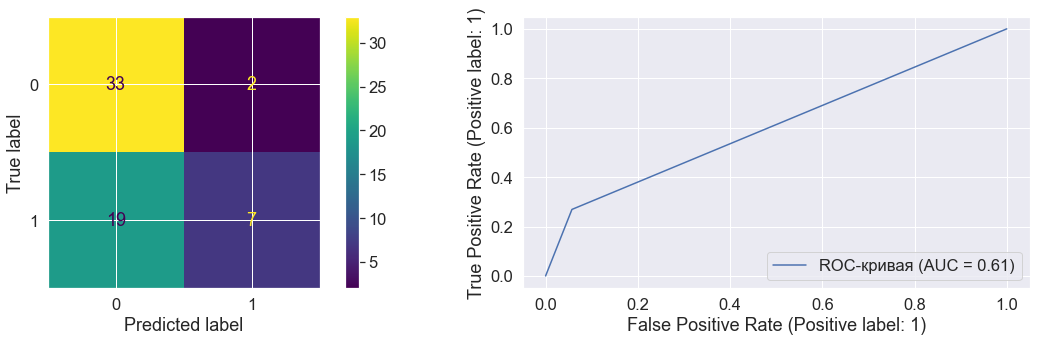
\includegraphics[width=\textwidth]{mysvm} 

Та же регрессия только с добавлением параметра lambda. 

\begin{alltt}
\{'lin\_\_alpha': 0.0001, 'lin\_\_max_iter': 1000\}
Accuracy train: 0.702295918367347
Accuracy: 0.6721311475409836
Recall: 0.5384615384615384
Precision: 0.6363636363636364
\end{alltt}
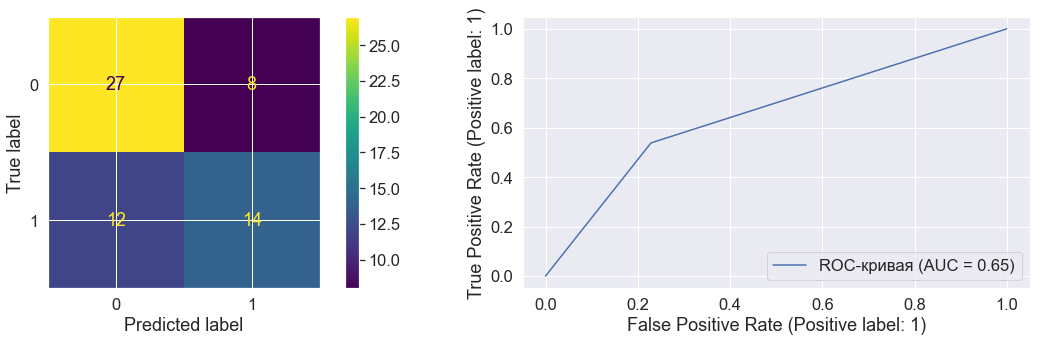
\includegraphics[width=\textwidth]{sklsvm}


\begin{lstlisting}[language=C]

\end{lstlisting}


После таких плохих результатов работы линейных моделей я попытался преобразовать данные. Точность увеличилась после добавления произведения двух лучше всего разделяемых параметров: thalachh и oldpeak и бинаризации категориальных параметров датасета. 


\CWHeader{Logistic Regression }

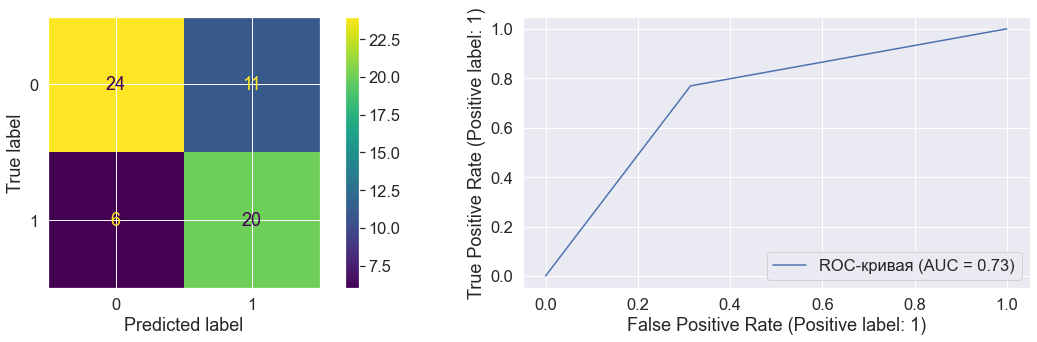
\includegraphics[width=\textwidth]{mylogup}
\begin{alltt}
\{'log\_\_batch\_size': 1, 'log\_\_lr': 0.1, 'log\_\_nepoch': 20\}
Accuracy train: 0.7147959183673469
Accuracy: 0.7213114754098361
Recall: 0.7692307692307693
Precision: 0.6451612903225806
\end{alltt}

\CWHeader{KNN}

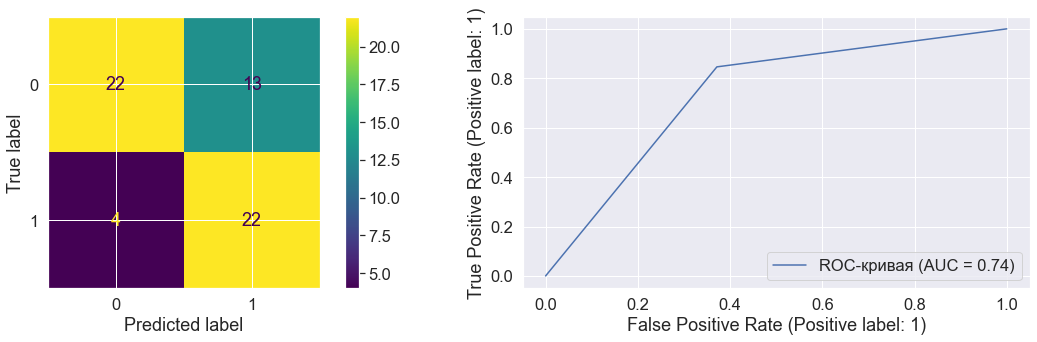
\includegraphics[width=\textwidth]{myknnup}
\begin{alltt}
\{'knn\_\_k': 22\}
Accuracy train: 0.7023809523809523
Accuracy: 0.7213114754098361
Recall: 0.8461538461538461
Precision: 0.6285714285714286
\end{alltt}

\CWHeader{NaiveBayes}

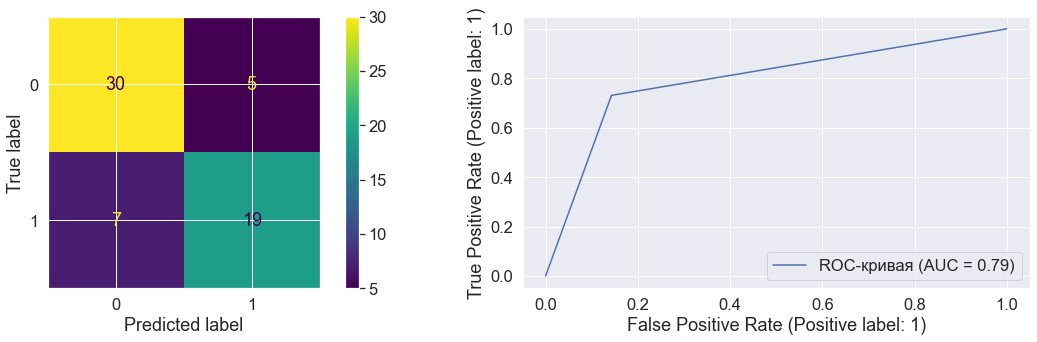
\includegraphics[width=\textwidth]{mynbup}
\begin{alltt}
\{'bn\_\_bins': 2\}
Accuracy train: 0.7894557823129251
Accuracy: 0.8032786885245902
Recall: 0.7307692307692307
Precision: 0.7916666666666666
\end{alltt}

\CWHeader{SVM}

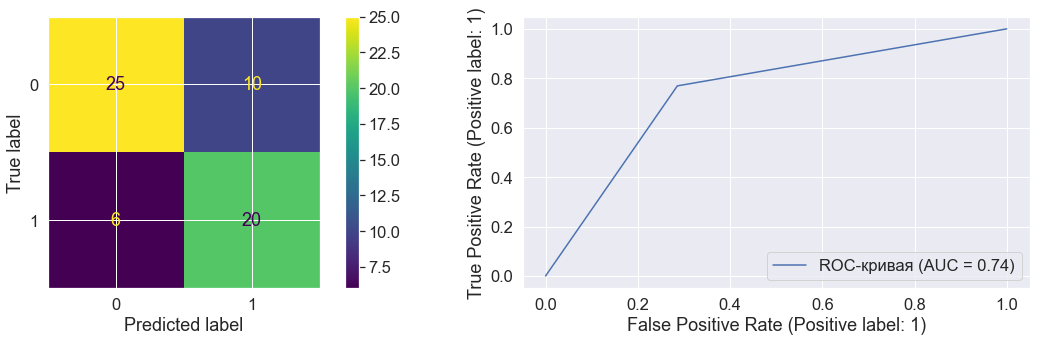
\includegraphics[width=\textwidth]{mysvmup}
\begin{alltt}
\{'lin\_\_batch\_size': 10, 'lin\_\_lambd': 0, 'lin\_\_lr': 0.1, 'lin\_\_nepoch': 20\}
Accuracy train: 0.7272108843537415
Accuracy: 0.7377049180327869
Recall: 0.7692307692307693
Precision: 0.6666666666666666
\end{alltt}



\pagebreak